\documentclass[epsfig,10pt,fullpage]{article}

\newcommand{\LabNum}{10}
\newcommand{\CommonDocsPath}{../../common/docs}
\input{\CommonDocsPath/preamble.tex}
\usepackage{amsmath}

\begin{document}

\centerline{\huge Embedded Systems}
~\\
\centerline{\huge Laboratory Exercise \LabNum}
~\\
\centerline{\large Image Processing}
~\\

\noindent
CPUs are general-purpose computational devices that are capable of a wide variety of tasks. 
This level of flexibility however, comes at a cost; CPUs are slower at some tasks than 
specialized devices. Because of this factor, some applications can execute more quickly if 
parts of the implementation run on a specialized device, such as a custom circuit in a
field-programmable gate array (FPGA). This approach, of offloading computation to a faster
device, is known as \textit{hardware acceleration}.

\noindent
~\\
In this laboratory exercise, we will implement two versions of an image processing application
that detects the edges of an image. The first version will run entirely on the CPU. This
discussion assumes that you are using the ARM processor in the DE1-SoC Computer to run your 
programs. If a different board is being used, the same instructions will mostly apply, but we 
will point out any differences as needed. The second version of the application will
make use of hardware acceleration, by offloading most of the image processing operations to 
a hardware accelerator implemented inside an FPGA. We will assume that image files are 
represented in the {\it bitmap} (BMP) file format, using {\it 24-bit true color}.

\noindent
\section*{The Canny Edge-Detection Technique}

\noindent
In this exercise, we will implement a variation of the \textit{Canny edge detector}, which is 
a widely-used edge-detection scheme. Figures~\ref{fig:tracks} and \ref{fig:tracks_edges} 
show a sample image that is provided as the input to a Canny edge detector, as well as the 
resulting edge-detected output image. 
As illustrated in Figure~\ref{fig:canny}, the Canny edge-detection algorithm involves five
stages that are applied to the input image in succession. The following 
sections describe each stage of the algorithm and show how the sample image from 
Figure~\ref{fig:tracks} is transformed as it passes through each stage.

~\\
~\\
\begin{figure}[h]
\centering
\begin{minipage}[b]{0.475\textwidth}
	\includegraphics[width=\textwidth]{figures/tracks.png}
	\caption{Original image.}
	\label{fig:tracks}
\end{minipage}
\hfill
\begin{minipage}[b]{0.475\textwidth}
	\includegraphics[width=\textwidth]{figures/tracks_edges.png}
	\caption{Edge-detected image.}
	\label{fig:tracks_edges}
\end{minipage}
\end{figure}
\pagebreak
\begin{figure}[H]
   \begin{center}
       \includegraphics[scale = 0.6]{figures/canny.pdf}
   \end{center}
	\caption{The Canny edge-detection algorithm.}
	\label{fig:canny}
\end{figure}

\noindent
\section*{Stage 1: Grayscale Conversion}

Figure~\ref{fig:sample_stage1} shows the state of our sample image at the end of the grayscale 
conversion stage. This stage converts the input 24-bit bitmap color image (8 bits each for red, 
green, and blue) into an 8-bit grayscale image. The grayscale value at each pixel is calculated 
as the average of the three 8-bit color values of the original image.

\begin{figure}[h]
   \begin{center}
       \includegraphics[scale = 0.85]{figures/fig_stage1_grayscale.png}
   \end{center}
   \caption{The sample input image after the grayscale conversion stage.}
	\label{fig:sample_stage1}
\end{figure}

\noindent
\section*{Stage 2: Gaussian Smoothing}

\begin{figure}[h]
   \begin{center}
       \includegraphics[scale = 0.85]{figures/fig_stage2_gaussian.png}
   \end{center}
   \caption{The sample input image after the Gaussian smoothing stage.}
	\label{fig:sample_stage2}
\end{figure}

The purpose of the Gaussian smoothing stage is to remove some of the ``noise'' in the image. Smoothing of
the image allows the edge-detection mechanism to focus on changes in image intensity that correspond to
features in the image, as opposed to random variations that can be attributed to image noise.
Figure~\ref{fig:sample_stage2} shows the state of our sample image at the end of the Gaussian 
smoothing stage. 

\noindent
Smoothing, or blurring, of the image is accomplished by using a {\it Gaussian filter}, which 
modifies noisy pixels (pixels that are unlike their neighbouring pixels) to be more like 
their neighbours. An example of a 2-D Gaussian function is illustrated in 
Figure~\ref{fig:gaussian}$a$. The shape of this function can be selected by choosing different 
values for the standard deviation $\sigma$. For this exercise we are using a 
digital version of the Gaussian, 
specified as a $5 \times 5$ filter, or {\it kernel}. This kernel corresponds to a Gaussian function
with standard deviation $\sigma = 1$ and mean $\mu = 0$. Part~($b$) of Figure~\ref{fig:gaussian}
shows how the kernel is applied to the image. The * operator denotes {\it convolution}, $A$ is 
the original image, and $B$ is the resulting filtered image.

\begin{figure}[h]
   \begin{center}
       \includegraphics[scale = 0.85]{figures/gaussian.pdf}
   \end{center}
   \caption{Gaussian functions and filters.}
	\label{fig:gaussian}
\end{figure}

%\[
%B = 1/273
%\begin{bmatrix}
    %1 & 4 & 7 & 4 & 1 \\
    %4 & 16 & 26 & 16 & 4 \\
    %7 & 26 & 41 & 26 & 7 \\
    %4 & 16 & 26 & 16 & 4 \\
    %1 & 4 & 7 & 4 & 1
%\end{bmatrix} * A
%\]

~\\
\noindent
For a pixel in row $i$, column $j$ of the image $A$, the kernel generates the dot-product
\begin{eqnarray*}
    B_{i, j}&=& (A_{i-2, j-2} + 4 A_{i-2, j-1} + 7 A_{i-2, j} + 4 A_{i-2, j+1} + A_{i-2, j+2} +\\
    &&4 A_{i-1, j-2} + 16 A_{i-1, j-1} + 26 A_{i-1, j} + 16 A_{i-1, j+1} + 4 A_{i-1, j+2} +\\
    &&7 A_{i, j-2} + 26 A_{i, j-1} + 41 A_{i, j} + 26 A_{i, j+1} + 7 A_{i, j+2} +\\
    &&4 A_{i+1, j-2} + 16 A_{i+1, j-1} + 26 A_{i+1, j} + 16 A_{i+1, j+1} + 4 A_{i+1, j+2} +\\
    &&A_{i+2, j-2} + 4 A_{i+2, j-1} + 7 A_{i+2, j} + 4 A_{i+2, j+1} + A_{i+2, j+2}) \div 273
\end{eqnarray*}

\noindent
The convolution operation performs this calculation for every pixel $i, j$ so that 
each resulting pixel $B_{i,j}$ gets assigned the weighted average value of $A_{i,j}$ and 
the $5 \times 5$ grid of pixels surrounding it (if a pixel is near the 
top/bottom or left/right of the image,
then 0's are inserted for any ``missing'' pixels that are needed for the calculation). Each 
dot-product result is divided by 273, which is the sum of the weights in the kernel, 
so that the overall intensity of pixels in the image does not change.

\noindent
\section*{Stage 3: Sobel Operator} 

The Sobel stage is used to identify {\it edges} in the image $B$ produced as the output of
the Gaussian stage. It works by finding changes in the image intensity in both the horizontal
(rows) and vertical (columns) directions. If we consider $B$ to be a two-dimensional
function $f(x,y)$, then changes in the image across each row are calculated by finding the 
{\it partial derivative} of the image in the $x$ direction, 
${\partial f}/{\partial x}$. Similarly, the partial derivative in the $y$ direction, 
${\partial f}/{\partial y}$, is used to find changes in the image along each column. To see 
how the partial derivatives can be calculated, consider the expressions in 
Figure~\ref{fig:derivative}. 

\begin{figure}[h]
   \begin{center}
       \includegraphics[scale = 0.85]{figures/derivative.pdf}
   \end{center}
   \caption{The calculation of partial derivatives.}
	\label{fig:derivative}
\end{figure}

~\\
\noindent
Part~($a$) of Figure~\ref{fig:derivative} gives the traditional expression for 
the derivative of a function $f^\prime(x)$, which is the limit as $h$ approaches~0 of 
$\Delta{f}/\Delta{x}$, where $\Delta{f}=f(x+h)-f(x)$ and $\Delta{x} = h$. To calculate the 
derivative of an image at each pixel it is better to use the modified expression in 
Figure~\ref{fig:derivative}$b$, in which $\Delta{f} = f(x+0.5h) - f(x-0.5h)$. Part~$c$ of 
the figure provides an example that illustrates how this expression applies to a pixel in a row 
of an image. To find the derivative of the pixel in the middle of the row (which has the 
intensity 200) we use the pixels immediately to the right and left. Thus, 
$\Delta{f} = 210 - 10$ and $\Delta{x} = 2$. The key idea for finding derivatives at each 
pixel in an image is expressed by the {\it derivative filter} shown on the right hand side 
of Figure~\ref{fig:derivative}$c$. It represents the calculation of $\Delta{f}$ and is used 
as the basis for the Sobel stage convolution described below.

~\\
\noindent
The Sobel stage uses convolution similar to the Gaussian stage, but with two different 
$3 \times 3$ kernels. The kernels and convolution operations are given below.

\[
\frac{\partial{f}}{\partial{x}} = 
\begin{bmatrix}
    -1 & 0 & 1  \\
    -2 & 0 & 2  \\
    -1 & 0 & 1 
\end{bmatrix} * B
\ \ \ \ \ \ \  \ \ \ \ \  \frac{\partial{f}}{\partial{y}} = 
\begin{bmatrix}
    1 & 2 & 1 \\
    0 & 0 & 0 \\
    -1 & -2 & -1
\end{bmatrix} * B
\]

~\\
\noindent
These kernels represent versions of the derivative filter, extended to two dimensions, that 
is derived in Figure~\ref{fig:derivative}. For each pixel, the value of 
${\partial{f}}/{\partial{x}}$ depends on three rows, where pixels in the same row are 
weighted by a factor of two. For example, $({\partial{f}}/{\partial{x}})_{i,j}$ for 
the pixel in row $i$, column $j$ is calculated as 

\begin{eqnarray*}
    \left(\frac{\partial{f}}{\partial{x}}\right)_{i, j}&=& B_{i-1, j+1} + 2 B_{i, j+1} + B_{i+1, j+1} -\\
    &&(B_{i-1, j-1} + 2 B_{i, j-1} + B_{i+1, j-1})
\end{eqnarray*}

~\\
\noindent
Similarly, the value of ${\partial{f}}/{\partial{y}}$ for each pixel depends on three
columns. Considered as a vector, the partial derivatives in the $x$ and $y$ directions
are referred to as the {\it intensity gradient}:

$$\nabla{f}=\left[\frac{\partial{f}}{\partial{x}},\frac{\partial{f}}{\partial{y}}\right]$$

~\\
\noindent
The {\it magnitude} of the intensity gradient at each pixel reflects whether that pixel is on an
``edge'' from the original image, and the {\it angle} of the gradient indicates the
direction of the corresponding edge. In this exercise we define the magnitude of the
gradient as the average of the absolute values of the partial derivatives: 

\begin{equation}
    \|\nabla{f}\|=\frac{1}{2}\left(\left|\frac{\partial{f}}{\partial{x}}\right|+\left|\frac{\partial{f}}{\partial{y}}\right|\right)
\end{equation}

~\\
\noindent
If Equation (1) generates a result that is too large to fit into a pixel's eight-bit grayscale
value, then the pixel is set to its maximum value of 255. The angle of the gradient is
defined by:

\begin{equation}
    \theta={tan}^{-1}\left(\frac{{\partial{f}}/{\partial{y}}}{{\partial{f}}/{\partial{x}}}\right)
\end{equation}

~\\
\noindent
The angle $\theta$ reflects the direction of greatest ascent (in the image) at the pixel. Thus,
if the pixel is on a horizontal edge then $\theta=\pm {90}^\circ$, and if the pixel is on a 
vertical edge then $\theta = 0^\circ$ or $\theta = {180}^\circ$.

~\\
\noindent
Figure~\ref{fig:sample_stage3} shows the results produced by the Sobel stage.
Parts ($a$) and ($b$) of the figure illustrate the partial derivatives and part ($c$)
shows the overall gradient. In these images the edges of the original image are highlighted 
as brighter pixels. Non-edges, which are areas with low intensity gradients, appear as 
darker pixels.

~\\
\begin{figure}[h]
\centering
\begin{minipage}[b]{0.32\textwidth}
	\includegraphics[width=\textwidth]{figures/stage2_gradient_x.png}
    \center{\sf{(a)} $\frac{\partial{f}}{\partial{x}}$}
\end{minipage}
\hfill
\begin{minipage}[b]{0.32\textwidth}
	\includegraphics[width=\textwidth]{figures/stage2_gradient_y.png}
    \center{\sf{(b)} $\frac{\partial{f}}{\partial{y}}$}
\end{minipage}
\hfill
\begin{minipage}[b]{0.32\textwidth}
   \includegraphics[width=\textwidth]{figures/fig_stage3_sobel.png}
    \center{\sf{(c)} $\nabla{f}$}
\end{minipage}
   \caption{Images representing the partial derivatives and the image gradient.}
	\label{fig:sample_stage3}
\end{figure}

~\\
\noindent
To illustrate the effect of the Sobel operator, let us examine different image boundaries that 
may exist in an image as shown in Figure~\ref{fig:image_boundaries}. For each $3 \times 3$
image shown, we can use the Sobel operator to calculate the intensity gradient at the center 
pixel. Let us examine the vertical example, where there is a boundary between darker 
pixels on the left side of the image and brighter pixels on the right side. In this 
example, ${\partial{f}}/{\partial{x}}$ of the center pixel can be calculated as 
$91 + 2(89) + 92 - (1 + 2(1) + 3) = 355$. In the vertical direction, ${\partial{f}}/{\partial{y}}$
is $1 + 2(49) + 91 -(3 + 2(46) + 92) = 3$. The intensity gradient for 
this pixel is high in the horizontal direction, and low in the vertical direction, which is to 
be expected along a vertical boundary. The overall intensity gradient is
$\nabla{f} = \frac{1}{2}(355 + 3) = 179$. This is a bright pixel value, meaning that
the Sobel operator has detected this boundary as a strong edge. The gradient angle $\theta
= 0^\circ$ because the direction of steepest ascent is left-to-right.

\begin{figure}[H]
   \begin{center}
       \includegraphics[scale = 1.0]{figures/edges.pdf}
   \end{center}
   \caption{Examples of edges in an image.}
	\label{fig:image_boundaries}
\end{figure}

~\\
\noindent
In the horizontal case given in Figure~\ref{fig:image_boundaries}, using
the Sobel operator to calculate the intensity gradient at the center we see that the 
vertical gradient is high (${\partial{f}}/{\partial{y}} = -364$) and the 
horizontal gradient is low (${\partial{f}}/{\partial{x}} =  2$). The angle $\theta =
-90^\circ$ because the direction of greatest ascent from darker to brighter pixels is
downward from the top of the image.  For each of the diagonal 
cases in Figure~\ref{fig:image_boundaries}, the gradients are high in both the $x$ and $y$ 
directions. The values of $\theta = \pm45^\circ$ represent the directions from darker to brighter
pixels in each image. Finally, for the non-boundary case, 
the gradients are low in both directions with ${\partial{f}}/{\partial{x}} = 1$ and 
${\partial{f}}/{\partial{y}} = 19$. As the gradients 
are low, the center pixel would become dark with a value of
$\nabla{f} = \frac{1}{2}(1 + 19) = 10$.

\noindent
\section*{Stage 4: Non-Maximum Suppression} 

\noindent
After the Sobel stage, some of the edges identified in the image may be thick and/or blurry. 
The non-maximum suppression stage is used to enhance and sharpen the edges by making them thinner. 
This stage examines each pixel in the image that is on an edge and 
compares the pixel with its neighbours that may be part of the same edge---if the pixel is 
brighter than its neighbours, then its intensity is retained, else it is set to 0.
Figure~\ref{fig:sample_stage4} shows the state of our sample image at the end of the 
non-maximum suppression stage. 

~\\
\begin{figure}[H]
   \begin{center}
       \includegraphics[scale = 0.85]{figures/fig_stage4_nonmax_suppression.png}
   \end{center}
   \caption{The sample input image after the non-maximum suppression stage.}
	\label{fig:sample_stage4}
\end{figure}

\begin{figure}[H]
   \begin{center}
       \includegraphics[scale = 0.8]{figures/fig_nonmaximum_suppression.pdf}
   \end{center}
   \caption{The effect of nonmaximum suppression on a blurred vertical line.}
	\label{fig:nonmaximum_suppression}
\end{figure}

~\\
\noindent
The effect of non-maximum suppression on a sample image containing a blurry vertical line 
is illustrated in Figure~\ref{fig:nonmaximum_suppression}.
The vertical line, which is originally three-pixels wide, becomes one-pixel
wide in the output image. Non-maximum suppression works by examining each pixel in the 
image in turn. The value of the gradient direction $\theta$ produced during the Sobel stage
for the pixel indicates the type of associated edge. If $\theta$ is 
close to $0^\circ$ or $180^\circ$ then the pixel 
is on a ``vertical'' edge. In this case, the non-maximum suppression algorithm compares the 
intensity of its left and right neighbours to the pixel. If its intensity is higher,
then the pixel is preserved in the output image from this stage, else it is set to~0.
Similarly, a pixel with $\theta$ near $\pm90^\circ$ is preserved if its intensity is
higher than the ones above and below it, and pixels with $\theta$ around $\pm45^\circ$
are preserved only if their intensity is greater than the appropriate neighbours that would 
be a part of the same ``diagonal'' edge.
Following this process for each pixel in the image has the effect of producing thinner edges.

\noindent
\section*{Stage 5: Hysteresis}

The goal of the hysteresis stage is to remove any pixel that does not belong to an edge.
Additionally, weak edges are erased altogether by removing any pixel that does not meet 
a user-defined intensity threshold. The hysteresis algorithm examines each pixel to determine 
whether: the pixel exceeds the user-defined threshold value, and there exists at least 
one adjacent pixel (horizontally, vertically, or diagonally) that exceeds the intensity threshold.
If both conditions are met, the pixel is preserved, else it is removed by turning it black. 
Figure~\ref{fig:sample_stage5} shows the end result of the hysteresis stage. 
 
\begin{figure}[H]
   \begin{center}
       \includegraphics[scale = 0.85]{figures/fig_stage5_hysteresis.png}
   \end{center}
   \caption{The sample input image after the hysteresis stage.}
	\label{fig:sample_stage5}
\end{figure}

\section*{Part I}

Write a C-language program that implements the five stages of the canny edge detector as described
above, and run your code on the DE1-SoC Computer. Some sample images are provided along
with this exercise. Sample skeleton code for this part is provided in Figure~\ref{fig:skeleton}. 
It contains functionality for loading and storing bitmap images. The {\it main} function for 
the program is given in part~($c$) of the figure. Once a 24-bit true-color image is loaded 
into memory, the code calls functions to transform the pixels according to the five 
edge-detection stages, and then writes the resulting image into an output file. The first 
step of edge-detection, in which the image is converted to grayscale, is provided in the code,
but you have to write the other stages.  The code in Figure~\ref{fig:skeleton} also 
shows how to measure the runtime of your program, which will allow you to compare with the 
hardware-accelerated version developed later in this exercise. The code in 
Figure~\ref{fig:skeleton} is provided along with this exercise. Some additional functionality not
shown in the figure is also included, such as code that can draw the images on an
output video display.  To view the images generated by your program, you can connect
a video monitor to your DE1-SoC board. Alternatively, you can view the images by using the
VGA emulator that is provided along with Lab Exercise 6. This emulator allows video output
to be displayed in a window within a VNC Viewer tool.


\lstset{language=C,numbers=none,escapechar=|,basicstyle=\small\ttfamily,}
\begin{figure}[h]
\begin{center}
\begin{minipage}[t]{15.5 cm}
\begin{lstlisting}[name=skeleton]
#include <stdio.h>
#include <stdlib.h>
#include <string.h>
#include <time.h>

int width, height; // the dimensions of the image
struct pixel {
    unsigned char b;
    unsigned char g;
    unsigned char r;
};

// Read BMP file and extract the pixel values (data) and header.
// Data is data[0] = BLUE, data[1] = GREEN, data[2] = RED, data[3] = BLUE, etc...
int read_bmp(char *filename, unsigned char **header, struct pixel **data) {
    struct pixel *data_tmp;
    unsigned char *header_tmp;
    FILE *file = fopen (filename, "rb");
    if (!file) return -1;
    
    // read the 54-byte header
    header_tmp = malloc (54 * sizeof(unsigned char));
    fread (header_tmp, sizeof(unsigned char), 54, file); 

    // get height and width of image from the header
    width = *(int*)(header_tmp + 18);  // width is a 32-bit int at offset 18
    height = *(int*)(header_tmp + 22); // height is a 32-bit int at offset 22

    // Read in the image
    int size = width * height;
    data_tmp = malloc (size * sizeof(struct pixel)); 
    fread (data_tmp, sizeof(struct pixel), size, file); // read the data
    fclose (file);
    
    *header = header_tmp;
    *data = data_tmp;
    return 0;
}
\end{lstlisting}
\end{minipage}
\caption{An outline of the software for edge detection (part $a$).}
\label{fig:skeleton}
\end{center}
\end{figure}

\lstset{language=C,numbers=none,escapechar=|}
\begin{center}
\begin{minipage}[t]{15.5 cm}
\begin{lstlisting}[name=skeleton]
// Set the grayscale 8-bit value by averaging the r, g, and b channel values.
// Store the 8-bit grayscale value in the r channel.
void convert_to_grayscale(struct pixel *data) {
    int x, y;
    
    // declare image as a 2-D array, to allow the syntax image[row][column]
    struct pixel (*image)[width] = (struct pixel (*)[width]) data;
    for (y = 0; y < height; y++) {          // y = 0 is the bottom row
        for (x = 0; x < width; x++) {       // x = 0 is the left side
            // Use the 8 bits of the r field to hold the grayscale image
            image[y][x].r = (image[y][x].r + image[y][x].b + image[y][x].g) / 3;
        }
    }
}

// Write the grayscale image to disk. The 8-bit grayscale values should be
// inside the r channel of each pixel.
void write_bmp(char *filename, unsigned char *header, struct pixel *data) {
    FILE* file = fopen (filename, "wb");
    // declare image as a 2-D array, to allow the syntax image[row][column]
    struct pixel (*image)[width] = (struct pixel (*)[width]) data;
    
    // write the 54-byte header
    fwrite (header, sizeof(unsigned char), 54, file); 
    int y, x;
    
    // the r field of the pixel has the grayscale value; copy to g and b.
    for (y = 0; y < height; y++) {          // y = 0 is the bottom row
        for (x = 0; x < width; x++) {       // x = 0 is the left side
            image[y][x].b = image[y][x].r;
            image[y][x].g = image[y][x].r;
        }
    }
    int size = width * height;
    fwrite (image, sizeof(struct pixel), size, file); // write the data
    fclose (file);
}

// Gaussian blur. Operate on the .r fields of the pixels only.
void gaussian_blur(|$\ldots$|) {
    unsigned int filter[5][5] = {
        { 1,  4,  7,  4, 1 },
        { 4, 16, 26, 16, 4 },
        { 7, 26, 41, 26, 7 },
        { 4, 16, 26, 16, 4 },
        { 1,  4,  7,  4, 1 }
    };
	 // ... code not shown
}

\end{lstlisting}
~\\
Figure \ref{fig:skeleton}. An outline of the software for edge detection (part $b$).
\end{minipage}
\end{center}

\lstset{language=C,numbers=none,escapechar=|}
\begin{center}
\begin{minipage}[t]{15.5 cm}
\begin{lstlisting}[name=skeleton]
void sobel_filter(|$\ldots$|) {
    int sobel_x[3][3] = {   // Sobel x direction (finds vertical edges)
        { -1,  0,  1 },
        { -2,  0,  2 },
        { -1,  0,  1 }
    };
    int sobel_y[3][3] = {   // Sobel in y direction (finds horizontal edges)
        { -1, -2, -1 },     // y == 0 (bottom) row
        {  0,  0,  0 },     // y == 1 (middle) row
        {  1,  2,  1 }      // y == 2 (top) row
    };
	 // ... code not shown
}

void non_maximum_suppressor(|$\ldots$|) {
	 // ... code not shown
}

void hysteresis_filter(|$\ldots$|) {
    #define strong_pixel_threshold 32	// example value
	 // ... code not shown
}

int main(int argc, char *argv[]) {
    struct pixel *image;     // used to hold the image after each stage
    signed int *G_x, *G_y;   // used to hold the partial derivatives after Sobel
    unsigned char *header;
    time_t start, end;
    
    if (argc < 2) {         // Check inputs
        printf("Usage: part1 <BMP filename>\n");
        return 0;
    }
    // Open input image file (24-bit true color bitmap)
    if (read_bmp (argv[1], &header, &image) < 0) {
        printf("Failed to read BMP\n");
        return 0;
    }
    start = clock ();   // Start measuring time
    
    convert_to_grayscale (image);
    // gaussian_blur (&image);
    // sobel_filter (&image, &G_x, &G_y);
    // non_max_suppress (&image, G_x, G_y);
    // hysteresis_filter (&image);
    
    end = clock();
    
    printf("TIME ELAPSED: %.0f ms\n", ((double) (end - start)) * 1000 / CLOCKS_PER_SEC);
    
    write_bmp ("edges.bmp", header, image);
    return 0;
}
\end{lstlisting}
~\\
Figure \ref{fig:skeleton}. An outline of the software for edge detection (part $c$).
\end{minipage}
\end{center}

\section*{Part II}

For Part I you used the DE1-SoC Computer system to run your program. For this part, you will 
use a different computer system, which is illustrated in Figure~\ref{fig:edge_detect_system}.
This system include an edge-detection mechanism that is implemented as a hardware circuit 
in the FPGA device. As indicated in the figure, the hardware edge-detection mechanism 
consists of five components that are connected in sequence. The first component is called
{\it Mem-to-Stream DMA}. This component is a {\it direct memory access} (DMA) controller that 
reads a 24-bit color image from memory. As the DMA reads these pixels, it
{\it streams} (sends in sequence) them to the {\it RGB24-to-Grayscale} color-space converter.
This converter implements stage one of the canny edge detector, converting the 24-bit color 
pixels into 8-bit grayscale pixels. The grayscale pixels are then streamed to the 
{\it Edge Detector} component, which implements stages two to five. The 
{\it Grayscale-to-RGB24} color-space converter then transforms the grayscale image back into 
the RGB24 format, which the {\it Stream-to-Mem DMA} then writes back into memory. 

~\\
\noindent
Figure~\ref{fig:edge_detect_system} shows two types of memory ports in the FPGA: an SDRAM
port, and an Onchip-memory port. The physical address ranges of these memories are
\texttt{0xC0000000} to \texttt{0xC3FFFFFF} for SDRAM and \texttt{0xC8000000} to
\texttt{0xC807FFFF} for Onchip memory. If you are using the DE1-SoC or DE10-Standard
boards, then the edge-detection mechanism and video-out port are connected to the SDRAM port.
If you are using the DE10-Nano board, then the edge-detection mechanism and video-out port 
are connected to the Onchip memory (the DE10-Nano board does not include SDRAM). When the 
SDRAM memory is being used, the edge-detection mechanism assumes that the image size is 
$640 \times 480$ pixels, and the image is stored in the memory starting at address
\texttt{0xC0000000}. The edge-detected output image is saved to the address \texttt{0xC2000000}.
When the Onchip memory is being used, the image size is $320 \times 240$ pixels. The
original image is stored at address \texttt{0xC8000000}, and the edge-detected result
{\it overwrites} the original and is therefore stored at the same address.

~\\
\noindent
The DMA controllers shown in Figure~\ref{fig:edge_detect_system}, as well as the video-out port, 
require that each pixel in memory is {\it word-aligned}. Every 32 bits in memory should store 
one pixel, where bits 31 to 24 are (unused) padding bits, 23 to 16 are the red component, 
15 to 8 are green, and 7 to 0 are blue. 

~\\
\noindent
For the DE1-SoC and DE10-Standard boards the video-out port is initialized to read pixel 
data starting at the address \texttt{0xC0000000} (SDRAM). On the DE10-Nano board the video-out
port is set up to read pixel data from the address \texttt{0xC8000000} (Onchip memory).

~\\
\begin{figure}[H]
   \begin{center}
       \includegraphics[scale = 1.0]{figures/edge_detect_system.png}
   \end{center}
   \caption{The components of the edge-detection system.}
	\label{fig:edge_detect_system}
\end{figure}

\newpage
\noindent Perform the following:

\begin{enumerate}
\item
Reconfigure the FPGA with the \textit{Edge\_Detector\_System.rbf} file. An easy way to
program the FPGA is to execute the Linux command \texttt{/home/root/misc/program\_fpga}
(a description of the FPGA programming process is provided in the appendix of the 
tutorial \textit{Using Linux on DE-series Boards}). For this part you will make use of only 
the video-out capability of the system; the edge-detection capability will be used in Part III.

\item
Consider the code in Figure~\ref{fig:part2}. It first calls {\it read\_bmp}, shown in 
Figure~\ref{fig:skeleton}$a$, to read a bitmap image from a file into a data structure. 
The code then generates virtual addresses that allow access to SDRAM memory at physical 
address \texttt{0xC0000000}, and the FPGA lightweight bridge at address \texttt{0xFF200000}
(for the DE10-Nano board you would need to use the Onchip memory instead of SDRAM).
The functions {\it open\_physical} and {\it map\_physical} use the {\it /dev/mem} mechanism 
and the Linux system function {\it mmap} to provide virtual memory mappings of physical 
addresses. More details are provided in the tutorial {\it Using Linux on DE-series Boards}.

\item
You are to write the function {\it memcpy\_consecutive\_to\_padded} to complete the code in 
Figure~\ref{fig:part2}. This function has to write a 32-bit value into the SDRAM buffer
corresponding to each 24-bit pixel in the image.

\item
Compile and test your code. Some sample images that have the correct dimensions are provided with
this lab exercise ($640 \times 480$ pixels for the DE1-SoC and DE10-Standard boards, and $320
\times 240$ for the DE10-Nano). With a video monitor connected to your DE-series board, you 
should see the bitmap image, upside down, on the video display. (Note that you cannot
view your images using the video emulator (provided with Lab Exercise 6) that was mentioned in 
Part I, as this emulator does not work with the system in Figure~\ref{fig:edge_detect_system}.)

\item
Write a function called {\it flip} that flips the image vertically before writing it into
the SDRAM buffer. Test your code to see that the image is now displayed right-side up.

\end{enumerate}

\lstset{language=C,numbers=none,escapechar=|,basicstyle=\small\ttfamily,}
\begin{figure}[h]
\begin{center}
\begin{minipage}[t]{15.5 cm}
\begin{lstlisting}[name=part2]
int main(int argc, char *argv[]){
   struct pixel *data;		// used to hold the image pixels
   byte *header;				// used to hold the image header
	int width, height;		// image size
   int fd = -1;				// used to open/read/etc. the image file
	void *SDRAM_virtual;
	void *LW_virtual;

	// Pointer to the DMA controller for the original image
   volatile unsigned int *mem_to_stream_dma = NULL;

   // Check inputs
   if (argc < 2){
      printf ("Usage: edgedetect <BMP filename>\n");
      return 0;
   }
   // Open input image file (24-bit bitmap image)
   if (read_bmp (argv[1], &header, &data, &width, &height) < 0){
      printf ("Failed to read BMP\n");
      return 0;
   }
	printf ("Image width = %d pixels, Image height = %d pixels\n", width, height);
   
   if ((fd = open_physical (fd)) == -1)   // Open /dev/mem
      return (-1);
   SDRAM_virtual = map_physical (fd, 0xC0000000, 0x03FFFFFF);
   LW_virtual = map_physical (fd, 0xFF200000, 0x00005000);
	if ((LW_virtual == NULL) || (SDRAM_virtual == NULL))
      return (0);

	// Set up pointer to edge-detection DMA controller
   mem_to_stream_dma = (volatile unsigned int *)(LW_virtual + 0x3100);
   *(mem_to_stream_dma+3) = 0; // Turn off edge-detection hardware DMA

   // Write the image to the memory used for video-out and edge-detection
   memcpy_consecutive_to_padded (data, SDRAM_virtual, width*height);

   free(header);
   free(data);
   
	unmap_physical (SDRAM_virtual, 0x03FFFFFF);	// release mem mapping
	unmap_physical (LW_virtual, 0x00005000);		// release mem mapping
	close_physical (fd);									// close /dev/mem
   
   return 0;
}
\end{lstlisting}
\end{minipage}
\caption{The software code for Part II.}
\label{fig:part2}
\end{center}
\end{figure}

\section*{Part III}

For this part you are to extend your program from Part II so that it makes use of the
hardware edge-detection mechanism. You will need to access the programming registers of
the DMA controllers, which are illustrated in Figure~\ref{fig:pixel_ctrl}. 
The register at the \texttt{Base} address is called the {\it Buffer} register, and the one 
at address \texttt{Base+4} is the {\it Backbuffer} register. Each of these registers stores 
the address of a memory buffer.  The \texttt{Buffer} register stores the address of the
buffer that is {\it currently} being used by the DMA controller.

~\\
\noindent
The operation of the DMA controller can be turned {\it off} by writing the value \texttt{0} 
into the {\it Status} register, at address \texttt{Base+12}. Writing the value \texttt{0x4} 
turns the DMA controller {\it on}, so that it performs transfers from/to memory starting at 
the address in the {\it Buffer} register.

~\\
\noindent
It is possible for software to directly write into the {\it Backbuffer} register to change 
its contents, but not the {\it Buffer} register. To change the {\it Buffer} register it is 
necessary to perform a {\it swap} operation, explained below.

~\\
\noindent
A buffer register swap is caused by writing the value \texttt{1} to the {\it Buffer}
register. This write operation does not directly modify the content of 
the {\it Buffer} register, but instead causes the contents of the {\it Buffer} 
and {\it Backbuffer} registers to be swapped. The swap operation does not happen right away;
it occurs at the end of the current DMA operation, when all pixels have been transferred.
Software can poll the value of the $S$ bit in the {\it Status} register to see when a DMA
operation has been completed (an entire image has been processed). Writing the value 1 into 
the {\it Buffer} register causes $S$ to be set to 1. Then, when the DMA operation is 
completed, $S$ is reset back to 0.

~\\
\noindent
The addresses of the programming registers for the three DMA controllers shown in 
Figure~\ref{fig:edge_detect_system} are given in Table~\ref{tab:DMA_addr}. The last two
columns in the table give the initial contents of 
the {\it Buffer} and {\it Backbuffer} registers for
each DMA. The columns labeled SDRAM and Onchip show the contents when the SDRAM memory or
Onchip memory are being used, respectively.  For the video-port DMA controller,
the {\it Buffer} address is set to the start of memory, and the {\it Backbuffer} address 
points to the start of the edge-detected image. Performing a swap operation allows either
the original image or the generated edge-detected image to be displayed.

\clearpage
\newpage
\begin{figure}[h!]
   \begin{center}
       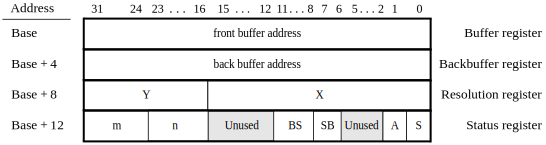
\includegraphics{figures/fig_DMA_ctrl.pdf}
   \end{center}
   \caption{DMA controller registers.}
	\label{fig:pixel_ctrl}
\end{figure}

\begin{table}[h]
\begin{center}
\begin{tabular}{l|c|l|c|c}
\textbf{DMA} & \textbf{Address} & \textbf{Register} & \textbf{SDRAM} & \textbf{Onchip}\\ \hline
 \rule{0cm}{12pt}Video-out & \texttt{0xFF203020} & Buffer & \texttt{0xC0000000} & \texttt{0xC8000000} \\
 & \texttt{0xFF203024} & Backbuffer & \texttt{0xC2000000} & \texttt{0xC8000000} \\
 & \texttt{0xFF203028} & Resolution &  & \\
 & \texttt{0xFF20302C} & Status &  & \\ \hline
 \rule{0cm}{12pt}Mem-to-Stream & \texttt{0xFF203100} & Buffer & \texttt{0xC0000000}
 & \texttt{0xC8000000} \\
 & \texttt{0xFF203104} & Backbuffer & \texttt{0xC0000000} & \texttt{0xC8000000} \\
 & \texttt{0xFF203108} & Resolution &  & \\
 & \texttt{0xFF20310C} & Status & & \\ \hline
 \rule{0cm}{12pt}Stream-to-Mem & \texttt{0xFF203120} & Buffer & \texttt{0xC2000000}
 & \texttt{0xC8000000} \\
 & \texttt{0xFF203124} & Backbuffer & \texttt{0xC2000000} & \texttt{0xC8000000} \\
 & \texttt{0xFF203128} & Resolution &  & \\
 & \texttt{0xFF20312C} & Status &  & \\
\end{tabular}
\caption{DMA register addresses.}
\label{tab:DMA_addr}
\end{center}
\end{table}

\noindent
Your program should do the following:
\begin{enumerate}
\item Disable the {\it Mem-to-Stream} and {\it Stream-to-Mem} DMA controllers. Recall that
you will first need to obtain virtual addresses for accessing the physical addresses in
Table~\ref{tab:DMA_addr}. Refer to the tutorial {\it Using Linux on DE-series Boards} if needed.
\item Copy the pixels of the input image to memory at address \texttt{0xC0000000}
(or \texttt{0xC8000000}).  The bitmap image should now appear on the video display.
\item Enable the DMAs to start the edge-detection operation. Then, perform a swap operation and 
wait until both DMA controllers are finished.
\item Disable the DMAs.
\item Perform a swap operation for the video DMA, so that the edge-detected image appears
on the display (not necessary for the DE10-Nano, because the result overwrites the original).
\item Save the edge-detected image into a file \textit{edges.bmp}, for later display. 
\item Test your program by using the images provided with this lab exercise. For the 
DE1-SoC and DE10-Standard boards $640 \times 480$ images are provided, and for the
DE10-Nano $320 \times 240$ images are included. Compare the run-time of your program with
the software-only solution from Part I, to see the benefits of using hardware acceleration.
\end{enumerate}

~\\
\noindent
\input{\CommonDocsPath/copyright.tex}

\end{document}
